\documentclass[9pt]{ctexbeamer}

\usepackage{pgfpages}

\makeatletter 
\def\beamer@framenotesbegin{% at beginning of slide
	\usebeamercolor[fg]{normal text}
}
\makeatother
%%%%%%%%%%%%%%%%%%

%%%%-----导入宏包-----%%%%
\usepackage{style/shubeamer}   % SHU 主题（含配色、帧标题、页脚、Python 代码样式）
\usepackage{amsmath,amsfonts,amssymb,bm}
\usepackage{graphicx,hyperref,url}
\usepackage{comment}
\usepackage{subcaption}
\usepackage{booktabs}
\usepackage{graphbox}
\usepackage{arydshln}
\usepackage[super,square]{natbib}
\usepackage{wrapfig} % 文字绕排
\usepackage{calligra}
%%%%%%%%%%%%%%%%%%

%%%%-----设置字体-----%%%%
\setmainfont{CMU Serif}
\setsansfont{CMU Sans Serif}
%%%%%%%%%%%%%%%%%%

\definecolor{nvidia}{RGB}{102,156,28}
\definecolor{red}{RGB}{184,13,73}
\definecolor{darkred}{RGB}{145,12,7}
\definecolor{orange}{RGB}{242,151,36}
\definecolor{darkteal}{RGB}{43,106,108}
\definecolor{darkgrey}{RGB}{64,64,64}
\definecolor{darkblue}{RGB}{4,37,58}
\definecolor{tan}{RGB}{225,221,191}
\definecolor{green}{RGB}{76,131,122}
\definecolor{darkgreen}{RGB}{42,50,46}
\definecolor{bluegray}{RGB}{33,36,39}
\definecolor{brown}{RGB}{110,54,42}

% 设置 Beamer 主题
\beamertemplateballitem
\AtBeginSection[]
{
	\begin{frame}<beamer>
		\frametitle{\textbf{目录}}
		\textbf{\tableofcontents[currentsection]}
	\end{frame}
}
%%%%%%%%%%%%%%%%%%



%%%%----设定图片存放路径
\graphicspath{{figures/}}

%%%%----首页信息设置----%%%% 方括号内容将显示在页脚
\AtBeginDocument{%
	%%%%----标题
	\title[Python金融数据分析]{\fontsize{16pt}{22pt}\selectfont {Python金融数据分析}}
	%%%%----副标题
	\subtitle{\fontsize{9pt}{14pt}\selectfont \textit{课程简介与引言}}
	%%%%----个人信息设置
	\author[王伟冠]{%
		\begin{tabular}{ll}%
			主讲人： & 王伟冠\tabularnewline%
			院\quad 系：   & 经济学院金融系\tabularnewline
			% \tabularnewline%
		\end{tabular}
	}
	%%%%----机构信息
	\institute[SHU]{上海大学}
	%%%%----日期信息
	\date[\today]{\today}}
%%%%----Macros for Vector, Matrix, Tensor, Math Operator and Misc
\input{style/macros.tex}
%%%%%%%%%%%%%%%%%%



\begin{document}

%% 封面信息，方括号内容是显示在页脚的短标题
\begin{frame}
	\titlepage
\end{frame}

%% 提纲页
\section*{目录}
\label{sec:toc}

\begin{frame}
	\frametitle{\textbf{目录}}
	\textbf{\tableofcontents}
\end{frame}


\section{课程简介与引言}

\begin{frame}{课程简介}
	\begin{itemize}
		\item 本课程旨在介绍Python在金融数据分析中的应用
		\item 学习Python的基本语法和常用库
		\item 通过案例分析，掌握金融数据分析的基本方法
	\end{itemize}
\end{frame}

\begin{frame}{课程信息}
	\begin{itemize}
		\item 课时数：24学时
		\item 教学方式：理论讲授+编程实践
		\item 考核方式：平时成绩：30\% 期末考试：70\%（开卷）
	\end{itemize}
	% insert two figures in one row
	\begin{figure}
		\centering
		\begin{subfigure}{0.3\textwidth}
			\centering
			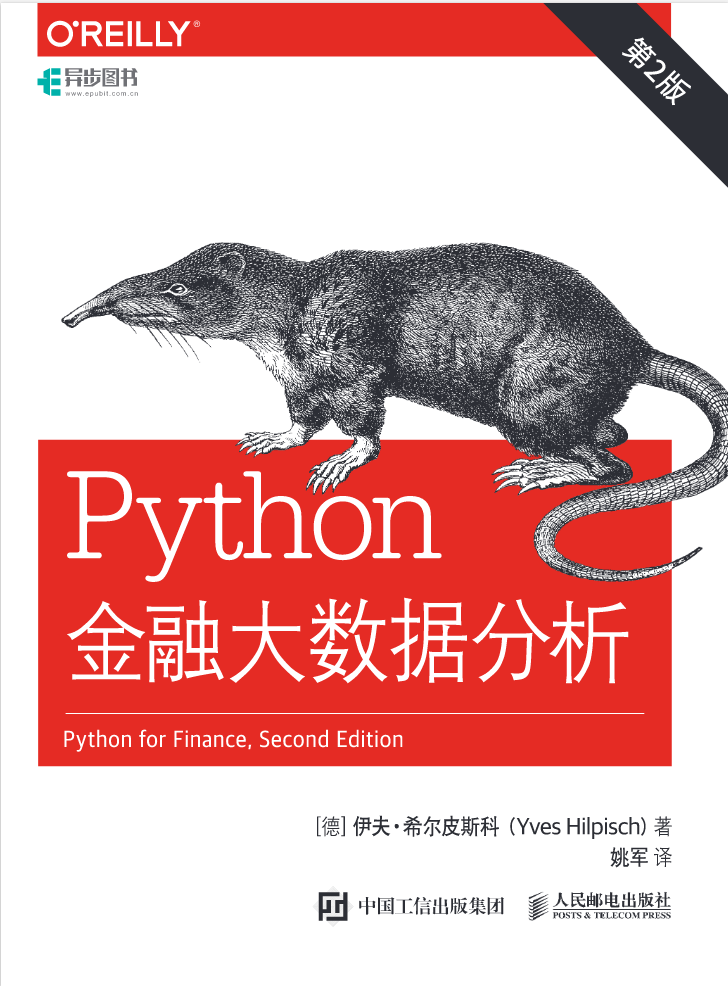
\includegraphics[width=0.8\linewidth]{figures/textbook1}
			\caption{主要教材。（陈旧）代码位置：\url{https://github.com/yhilpisch/py4fi2nd}}
		\end{subfigure}
		\hfill
		\begin{subfigure}{0.3\textwidth}
			\centering
			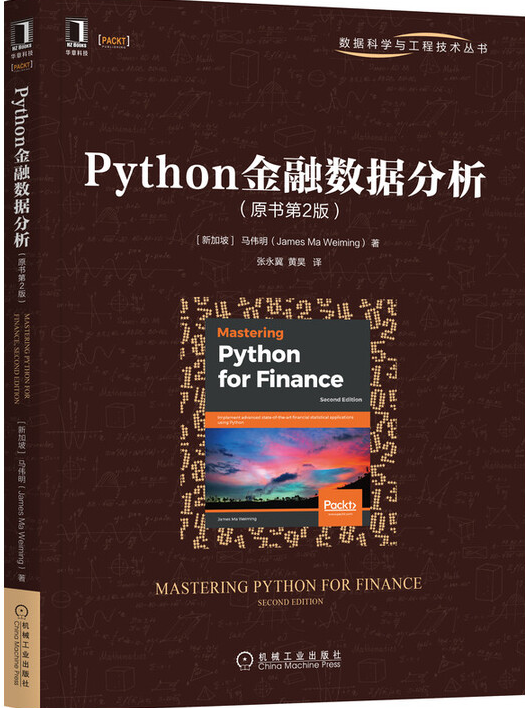
\includegraphics[width=0.8\linewidth]{figures/textbook2}
			\caption{辅助教材}
		\end{subfigure}
		\hfill
		\begin{subfigure}{0.3\textwidth}
			\centering
			
\includegraphics[width=0.8\linewidth]{figures/group-qr-code}
			\caption{课程群}
		\end{subfigure}
	\end{figure}
\end{frame}


\begin{frame}{课程安排}

	\begin{itemize}
		\item 为什么在金融中使用Python?
		\item Python的安装，IDE和虚拟环境
		\item Python的基本数据类型和结构
		\item Numpy和Pandas
		\item 可视化
		\item 金融时间序列数据分析
		\item 基本数学方法
		\item 统计学（投资组合优化）
		\item 面向对象的程序设计
		\item 其他（机器学习或其他案例）
	\end{itemize}
\end{frame}


\section{Python为什么变得如此重要？}

\begin{frame}{金融行业的数字化转型}
    \begin{itemize}
        \item 金融机构在大数据和实时决策的驱动下加速数字化，Python提供从数据接入到建模的完整链条。
        \item 开源生态降低试错成本，帮助团队快速迭代策略、风险模型与数据产品。
        \item Python脚本化特性让业务人员能够直接落地想法，缩短从洞察到部署的周期。
    \end{itemize}
\end{frame}

\begin{frame}{生态系统与工具链优势}
    \begin{itemize}
        \item pandas、NumPy、Polars 等高性能数据处理库适配结构化与半结构化金融数据。
        \item statsmodels、scikit-learn、PyTorch 为风险评估、量化策略和智能投顾提供建模基础。
        \item 与 SQL、Excel、Bloomberg API、REST 等系统的无缝集成，便于打通内部系统与外部数据源。
    \end{itemize}
\end{frame}

\begin{frame}{典型应用场景}
    \begin{columns}[T,totalwidth=\textwidth]
        \begin{column}{0.48\textwidth}
            \textbf{前台业务}
            \begin{itemize}
                \item 日内交易的策略回测与执行。
                \item 投资组合优化与风险预算。
                \item ESG、另类数据等主题投资的因子挖掘。
            \end{itemize}
        \end{column}
        \begin{column}{0.48\textwidth}
            \textbf{中后台}
            \begin{itemize}
                \item 市场、信用、流动性风险监控的自动化报告。
                \item 反洗钱与欺诈识别的机器学习模型。
                \item 监管合规、压力测试与情景分析的批量计算。
            \end{itemize}
        \end{column}
    \end{columns}
\end{frame}

\begin{frame}{人才与社区驱动}
    \begin{itemize}
        \item 全球量化基金、投行与金融科技公司广泛采用Python，形成“业界事实标准”。
        \item 丰富的在线社区、开源项目和教育资源，为从业者提供快速学习与问题解决渠道。
        \item 与 Jupyter、Airflow、Docker 等工具结合，支持端到端的协作开发、部署与运维。
    \end{itemize}
\end{frame}




\begin{frame}{生态系统和科学栈}
	\begin{itemize}
		\item NumPy 提供多维数组对象,以存储同构或者异构数据;它还提供操作这一数组对 象的优化函数/方法。  \item SciPy 是子库和函数的集合,它可以实现科学或者金融中常常用到的重要标准功能; 例如,你可以找到 3 次样条插值和数值积分的函数。
		\item Matplotlib 是非常流行的 Python 绘图和可视化库,提供 2D 和 3D 可视化功能。
		\item pandas 在 NumPy 基础上构建,可提供更丰富的时间序列和表格数据的管理与分析; 它与 Matplotlib 在绘图上
		\item scikit-learn 是流行的机器学习(ML)程序库,为许多不同的 ML 算法(如估值、 分类或者聚类)提供统一的应用编程接口(API)。
	\end{itemize}
	
\end{frame}


\section{为什么还要学习 Python 金融数据分析？}

\begin{frame}{AI 时代的思考}
  \begin{itemize}
    \item 如今，大语言模型（ChatGPT、Claude、Copilot 等）已经能够快速生成代码。
    \item 那么，为什么我们仍然需要学习这门课？
    \item 本课程不仅仅是“学写代码”，而是学习：
    \begin{enumerate}
      \item 金融数据的特点与经济含义
      \item 分析流程与研究规范
      \item 如何检验与解释模型结果
    \end{enumerate}
  \end{itemize}
\end{frame}

\begin{frame}{为什么不能完全依赖 AI 写代码？}
  \begin{itemize}
    \item AI 生成的代码往往是“黑箱”——需要你具备判断对错的能力。
    \item 金融数据复杂多变，AI 可能无法理解特定业务逻辑。
    \item 研究生、从业者需要：
    \begin{itemize}
      \item 能看懂代码与结果
      \item 知道哪里可能出错
      \item 会结合金融理论进行解释
    \end{itemize}
  \end{itemize}
\end{frame}

\begin{frame}{在学习本课程时应如何调整侧重点？}
  \begin{itemize}
    \item 不再把“记语法”作为重点，而是关注：
    \begin{enumerate}
      \item 如何提出金融问题（What is the research/analysis question?）
      \item 如何选择合适的工具与方法（Which model / which data?）
      \item 如何解读结果（金融意义、风险、投资价值）
    \end{enumerate}
    \item 将 AI 当作“助手”，而不是“替代品”。
    \item 真正的核心能力在于：\textbf{问题定义 + 方法论 + 批判性思维}。
  \end{itemize}
\end{frame}


\section{虚拟环境搭建}

\begin{frame}{为什么要使用虚拟环境？}
	\begin{itemize}
		\item 避免包版本冲突：不同项目可能需要不同版本的库，虚拟环境可以隔离这些依赖。
		\item 保持系统整洁：避免在全局环境中安装过多包，减少系统维护难度。
		\item 便于项目管理：每个项目可以有独立的环境，方便迁移和部署。
	\end{itemize}
\end{frame}

\begin{frame}{常用的虚拟环境工具}
	\begin{itemize}
		\item venv：Python 自带的虚拟环境工具，适合简单项目。
		\item virtualenv：功能更强大，支持更多 Python 版本。
		\item conda：不仅是虚拟环境管理器，还能管理包和依赖，适合数据科学项目。
		\item uv: 轻量级虚拟环境工具，适合快速创建和切换环境。
	\end{itemize}
\end{frame}



\begin{frame}[fragile]
\frametitle{使用 conda 构造虚拟环境}

\begin{itemize}
	\item 打开anaconda power shell
	\item 进入项目文件夹: 
	\begin{verbatim}
cd D:\<your_path>   # 注意路径上不要出现中文，容易出错
\end{verbatim}
  \item 创建环境：
  
  \begin{lstlisting}[language=python]
# 创建虚拟环境，Python 版本可根据需要调整
conda create -p ./.venv python=3.13  
#第一次运行需要接受条款，按a  
  \end{lstlisting}

  \item 激活环境：
  
  \begin{lstlisting}[language=python]
conda activate ./.venv
  \end{lstlisting}

  \item 展示已安装包：
  \begin{lstlisting}[language=python]
conda list
  \end{lstlisting}

  \item 安装所需包：
  \begin{lstlisting}[language=python]
conda install numpy pandas matplotlib scikit-learn -y
  \end{lstlisting}
\end{itemize}

\end{frame}


\begin{frame}
	\begin{itemize}
		\item 在VSCode中运行jupyter notebook格式的python代码，第一次需要安装python插件以及ipykernel
		\item 如果不能自动安装的话，在anaconda powershell中激活相应的虚拟环境以后安装。
		\item  报错显示某些包不存在
		\begin{figure}
		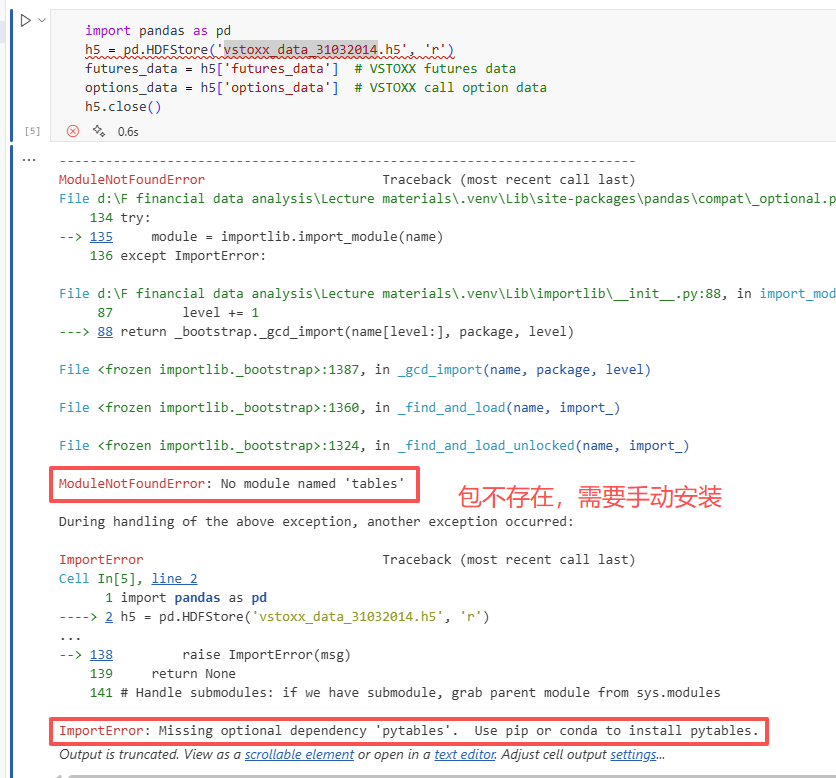
\includegraphics[width=0.6\textwidth]{missing-package.png}
	\end{figure}
	\end{itemize}


\end{frame}



%-----------------------------------------------------
\appendix



\begin{frame}[allowframebreaks]{参考文献}
	\bibliographystyle{style/gbt7714-2005}
	\bibliography{reference.bib} 
\end{frame}

\begin{frame}
	\begin{center}
		{\Huge\calligra Thanks for your attention!}
		\vspace{1cm}
		
		{\Huge Q \& A}
	\end{center}
\end{frame}
\end{document}

